\chapter{File formats}
\label{chap-file-formats}
\index{File!formats}
This chapter presents the formats of files read or generated by Unitex. The
formats of the DELAS and DELAF dictionaries have already been presented in
sections \ref{section-DELAF-format} and \ref{section-DELAS-format}.

\bigskip
\noindent NOTE: In this chapter the symbol \P ~represents the newline symbol.
Unless otherwise indicated, all text files described in this chapter are encoded
in Unicode Little-Endian.

\section{Unicode encoding}
\label{unicode-encoding}
\index{File!text}\index{Unicode}\index{File!\verbc{.txt}}\index{File!\verbc{.snt}}
By default, text files processed by Unitex have to be encoded in Unicode Little-Endian.
Unitex accepts also Unicode Big-Endian or UTF-8 files.
This encoding allows the representation of 65536 characters by coding each of
them in 2 bytes. In Little-Endian, the bytes are in lo-byte hi-byte order. If
this order is reversed, we speak of Big-Endian. A text file encoded in Unicode
Little-Endian, Big-Endian or UTF-8 starts with the special character (Unicode Byte Order Mark - BOM) with the hexadecimal value
\verb+FF+\,\verb+FE+ (Little-Endian), \verb+FE+\,\verb+FF+ (Big-Endian) or \verb+EF+\,\verb+BB+\,\verb+BF+ (UTF-8). 
Because UTF-8 has no byte order, adding a UTF-8 BOM is optional; for UTF-16 it is required.
The newline symbols have to be encoded by the two characters \verb+0D+\,\verb+00+ and \verb+0A+\,\verb+00+ (Little-Endian), 
\verb+00+\,\verb+0D+ and \verb+00+\,\verb+0A+ (Big-Endian), or \verb+0D+ and \verb+0A+ (UTF-8).

\bigskip
\noindent Consider the following text:

\bigskip
\texttt{Unitex\P}

\texttt{$\beta$-version\P}

\bigskip
\noindent Here is its representation in Unicode Little-Endian:

\bigskip
\begin{table}[!ht]
\begin{center}
\begin{tabular}{|c|c|c|c|c|c|c|c|c|}
\hline
BOM header & U & n & i & t & e & x & \P & $\beta$
\\
\hline
\verb+FF+\,\verb+FE+ & \verb+55+\,\verb+00+ & \verb+6E+\,\verb+00+ & \verb+69+\,\verb+00+ & \verb+74+\,\verb+00+ & \verb+65+\,\verb+00+ & \verb+78+\,\verb+00+
& \verb+0D+\,\verb+00+\,\verb+0A+\,\verb+00+ & \verb+B2+\,\verb+03+
\\
\hline
\hline
- & v & e & r & s & i & o & n & \P
\\
\hline
\verb+2D+\,\verb+00+ & \verb+76+\,\verb+00+ & \verb+65+\,\verb+00+ & \verb+72+\,\verb+00+ & \verb+73+\,\verb+00+ & \verb+69+\,\verb+00+ & \verb+6F+\,\verb+00+
& \verb+6E+\,\verb+00+ & \verb+0D+\,\verb+00+\,\verb+0A+\,\verb+00+
\\
\hline
\end{tabular}
\caption{Hexadecimal representation of a Unicode Little-Endian text}
\end{center}
\end{table}
\pagebreak
\bigskip
\noindent Here is its representation in Unicode Big-Endian:

\bigskip
\begin{table}[!ht]
\begin{center}
\begin{tabular}{|c|c|c|c|c|c|c|c|c|}
\hline
BOM header & U & n & i & t & e & x & \P & $\beta$
\\
\hline
\verb+FE+\,\verb+FF+ & \verb+00+\,\verb+55+ & \verb+00+\,\verb+6E+ & \verb+00+\,\verb+69+ & \verb+00+\,\verb+74+ & \verb+00+\,\verb+65+ & \verb+00+\,\verb+78+
& \verb+00+\,\verb+0D+\,\verb+00+\,\verb+0A+ & \verb+03+\,\verb+B2+
\\
\hline
\hline
- & v & e & r & s & i & o & n & \P
\\
\hline
\verb+00+\,\verb+2D+ & \verb+00+\,\verb+76+ & \verb+00+\,\verb+65+ & \verb+00+\,\verb+72+ & \verb+00+\,\verb+73+ & \verb+00+\,\verb+69+ & \verb+00+\,\verb+6F+
& \verb+00+\,\verb+6E+ & \verb+00+\,\verb+0D+\,\verb+00+\,\verb+0A+
\\
\hline
\end{tabular}
\caption{Hexadecimal representation of a Unicode Big-Endian text}
\end{center}
\end{table}

\bigskip
\noindent Here is its representation in Unicode UTF-8:

\bigskip
\begin{table}[!ht]
\begin{center}
\begin{tabular}{|c|c|c|c|c|c|c|c|c|}
\hline
BOM header & U & n & i & t & e & x & \P & $\beta$
\\
\hline
\verb+EF+\,\verb+BB+\,\verb+BF+ & \verb+55+ & \verb+6E+ & \verb+69+ & \verb+74+ & \verb+65+ & \verb+78+
& \verb+0D+\,\verb+0A+ & \verb+CE+\,\verb+B2+
\\
\hline
\hline
- & v & e & r & s & i & o & n & \P
\\
\hline
\verb+2D+ & \verb+76+ & \verb+65+ & \verb+72+ & \verb+73+ & \verb+69+ & \verb+6F+
& \verb+6E+ & \verb+0D+\,\verb+0A+
\\
\hline
\end{tabular}
\caption{Hexadecimal representation of a Unicode UTF-8 text}
\end{center}
\end{table}

\bigskip
\noindent On Unicode Little-Endian, the hi-bytes and lo-bytes have been reversed, which explains why the
start character is encoded as \verb+FF+\,\verb+FE+ in stead of \verb+FE+\,\verb+FF+, and
\verb+00+\,\verb+0D+ and \verb+00+\,\verb+0A+ are \verb+0D+\,\verb+00+ and \verb+0A+\,\verb+00+ respectively.



\section{Alphabet files}
There are two kinds of alphabet files: a file which defines the characters of a
language, and a file that indicates the sorting preferences. The first is
designed under the name \textit{alphabet}, the second under the name
\textit{sorted alphabet}.


\subsection{Alphabet}
\index{Alphabet}
The alphabet file is a text file that describes all characters of a language, as
well as the correspondances between capitalized and non-capitalized letters. This
file is called \verb+Alphabet.txt+ \index{File!\verbc{Alphabet.txt}} and is found
in the root of the directory of a language. Its presence is obligatory for Unitex
to function.

\bigskip
\noindent Example: the English alphabet file has to be in the directory
\verb+.../English/+

\bigskip
\noindent Each line of the alphabet file must have one of the following
three forms, followed by a newline symbol:

\begin{itemize}
  \item 
\includegraphics[height=0.5cm]{resources/img/korean_letters.png} : a
  hash symbol followed by two characters $X$ and $Y$ which indicate that all characters between $X$ and $Y$
  are letters. All these characters are considered to be in non-capitalized and
  capitalized form at the same time. This method is used to define the alphabets
  of Asian languages like Korean, Chinese or Japanese where there is no
  distinction between upper- and lower-case, and where the number of characters
  makes a complete enumeration tedious;

  \item \verb+Aa+ : two characters $X$ and $Y$ indicate that $X$ and $Y$ are
  letters and that $X$ is a capitalized equivalent of the non-capitalized $Y$
  form.

  \item 
\includegraphics[height=0.3cm]{resources/img/thai_letter.png}: a unique
  character $X$ defines $X$ as a letter in capitalized and non-capitalized form. This form is used to define a
  single Asian character.
\end{itemize}

\bigskip
\noindent For certain languages like French, it is possible that a lower-case
letter corresponds to multiple upper-case letters. For example, \texttt{\'e}, in
practice, can have the upper-case form \verb+E+ or \texttt{E}. To express
this, it suffices to use multiple lines. The reverse is equally true: a capitalized letter
can correspond to multiple lower-case letters. Thus, \verb+E+ can be the
capitalization of \verb+e+, \texttt{\'e}, \texttt{\`e}, \texttt{\"e} or
\texttt{\^e}. Here is an excerpt of the French alphabet file which defines different properties of letter
\verb+e+:

\bigskip
\noindent
\texttt{Ee}\P

\noindent
\texttt{E\'e}\P

\noindent
\texttt{\'E\'e}\P

\noindent
\texttt{E\`e}\P

\noindent
\texttt{\`E\`e}\P


\noindent
\texttt{E\"e}\P

\noindent
\texttt{\"E\"e}\P

\noindent
\texttt{E\^e}\P

\noindent
\texttt{\^E\^e}\P

\subsection{Sorted alphabet}
\index{Alphabet!sorted}
The sorted alphabet file defines the sorting priorities of the letters of a
language. It is used by the \verb+SortTxt+
program.\index{\verbc{SortTxt}}\index{External programs!\verbc{SortTxt}} Each line
of that file defines a group of letters. If a group of letters $A$ is defined
before a group of letters $B$, every letter of group $A$ is inferior to every
letter in group $B$.

\bigskip
\noindent The letters of a group are only distinguished if necessary. For example if the
group of letters \texttt{e\'e\`e\"e\^e} has been defined, the word
\texttt{\'ebahi} should be considered 'smaller' than \verb+estuaire+, and also
'smaller' than \texttt{\'et\'e}. Since the letters that follow
\verb+e+ and \texttt{\'e} determine the order of the words, it is
not necessary to compare letters \verb+e+ and \texttt{\'e} since they
are of the same group. On the other hand, if the words
\texttt{chant\'es} and \verb+chantes+ are to be sorted,
\verb+chantes+ should be considered as 'smaller'. It is therefore 
necessary to compare the letters \verb+e+ and \texttt{\'e} to
distinguish these words. Since the letter \verb+e+ appears first in the 
group \texttt{e\'e\`e\"e\^e}, it is considered to be 'smaller' than \texttt{chant\'es}. The word
\verb+chantes+ should therefore be considered to be 'smaller' than the word
\texttt{chant\'es}.

\bigskip
\noindent The sorted alphabet file allows the definition of equivalent characters.
It is therefore possible to ignore the different accents as well as
capitalization. For example, if the letters \verb+b+, \verb+c+, and \verb+d+ are
to be ordered without considering capitalization and the cedilla, it is possible
to write the following lines:

\bigskip
\noindent
\texttt{Bb}\P

\noindent
\texttt{Cc\c{C}\c{c}}\P

\noindent
\texttt{Dd}\P

\bigskip
\noindent This file is optional. If no sorted alphabet file is specified, the
\verb+SortTxt+ program sorts in the order of the Unicode encoding.


\section{Graphs}
\index{Graph!format}
This section presents the two graph formats: the graphic format \verb+.grf+ and
the compiled format \verb+.fst2+.


\subsection{Format .grf}
\index{File!\verbc{.grf}}
A \verb+.grf+ file is a text file that contains presentation information in
addition to information representing the contents of the boxes and the
transitions of the graph. A \verb+.grf+ file begins with the following lines:

\bigskip
\verb+#Unigraph+\P

\verb+SIZE 1313 950+\P

\verb+FONT Times New Roman:  12+\P

\verb+OFONT Times New Roman:B 12+\P

\verb+BCOLOR 16777215+\P

\verb+FCOLOR 0+\P

\verb+ACOLOR 12632256+\P

\verb+SCOLOR 16711680+\P

\verb+CCOLOR 255+\P

\verb+DBOXES y+\P

\verb+DFRAME y+\P

\verb+DDATE y+\P

\verb+DFILE y+\P

\verb+DDIR y+\P

\verb+DRIG n+\P

\verb+DRST n+\P

\verb+FITS 100+\P

\verb+PORIENT L+\P

\verb+#+\P

\bigskip
\noindent The first line \verb+#Unigraph+ is a comment line. The following lines
define the parameter values of the graph presentation:

\begin{itemize}
  \item \verb+SIZE x y+ : defines the width \verb+x+ and the hight \verb+y+ of a graph in pixels;
  
  \item \verb+FONT name:xyz+ : defines the font used for displaying the contents
  of the boxes. \verb+name+ represents the name of the mode. \verb+x+ indicates
  if the text should be in bold face or not. If \verb+x+ is \verb+B+, it
  indicates that it should be bold. For non-bold face, \verb+x+ should be a
  space. In the same way, \verb+y+ has value \verb+I+ if the text should be
  italic, a space if not. \verb+z+ represents the size of the text;

  \item \verb+OFONT name:xyz+ : defines the mode used for displaying transducer
  outputs. Parameters \verb+name+, \verb+x+, \verb+y+, and \verb+z+ are defined
  in the same way as \verb+FONT+;
  
  \item \verb+BCOLOR x+ : defines the background color of the graph. 'x'
  represents the color in RGB format;

  \item \verb+FCOLOR x+ : defines the foreground color of the graph. 'x'
  represents the color in RGB format;

  \item \verb+ACOLOR x+ : defines the color inside the boxes that correspond to
  the calls of sub-graphs. \verb+x+ represents the color in RGB format;

  \item \verb+SCOLOR x+ :  defines the color used for writing in comment boxes
  (boxes that are not linked up with any others). \verb+x+ represents the color
  in RGB format;

  \item \verb+CCOLOR x+ : defines the color used for designing selected boxes.
  \verb+x+ represents the color in RGB format;

  \item \verb+DBOXES x+ : this line is ignored by Unitex. It is conserved to
  ensure compatibility with Intex graphs;

  \item \verb+DFRAME x+ : there will be a frame around the graph if \verb+x+ is
  \verb+y+, not if it is \verb+n+;

  \item \verb+DDATE x+ : puts the date at the bottom of the graph if \verb+x+ is
  \verb+y+, not if it is \verb+n+;

  \item \verb+DFILE x+ : puts the name of the file at the bottom of the graph
  depending on whether \verb+x+ is \verb+y+ or \verb+n+;

  \item \verb+DDIR x+ : prints the complete path of the graph wether \verb+x+ is
  \verb+y+ or \verb+n+. This option has no effect if the \verb+DFILE+ option is
  set to \verb+n+;

  \item \verb+DRIG x+ : displays the graph from right to left or left to right
  depending on whether \verb+x+ is \verb+y+ or \verb+n+;

  \item \verb+DRST x+ : this line is ignored by Unitex. It isconserved to ensure
  compatibility with Intex graphs;

  \item \verb+FITS x+ : this line is ignored by Unitex. It isconserved to ensure
  compatibility with Intex graphs;

  \item \verb+PORIENT x+ : this line is ignored by Unitex. It isconserved to
  ensure compatibility with Intex graphs;

  \item \verb+#+ : this line is ignored by Unitex. It serves to indicate the end
  of the header information.
\end{itemize}

\bigskip
\noindent The lines after the header give the contents and the position of the
boxes in the graph. The following example corresponds to a graph recognizing a
number:

\bigskip
\verb+3+\P

\verb+"<E>" 84 248 1 2 +\P

\verb+"" 272 248 0 +\P

\verb$s"1+2+3+4+5+6+7+8+9+0" 172 248 1 1 $\P

\bigskip
\noindent The first line after the header indicates the number of boxes in the
graph, immediately followed by a newline. This number can not be lower than 2,
since a graph always has an initial and a final state.

\bigskip
\noindent The following lines define the boxes of the graph. The boxes are numbered
starting at $0$. By convention, state $0$ is the initial state and state $1$ is
the final state. The contents of the final state is always empty.

\bigskip
\noindent Each box in the graph is defined by a line that has the
following format:

\bigskip
\textit{contents X Y N transitions \P}

\bigskip
\noindent \textit{contents} is a sequence of characters enclosed in quotation
marks that represents the contents of the box. This sequence can sometimes be
preceded by an \verb+s+ if the graph is imported from Intex; this character is
then ignored by Unitex. The contents of the sequence is the text that has been
entered in the editing line of the graph editor. Table \ref{table10-2} shows the
encoding of two special sequences that are not encoded in the same way as they
are entered into the \verb+.grf+ files:

\bigskip
\begin{table}[!ht]
\begin{center}
\begin{tabular}{|c|c|}
\hline
Sequence in the graph editor & Sequence in the \verb+.grf+ file
\\
\hline
\verb$"$ & \verb$\"$
\\
\hline
\verb$\"$ & \verb$\\\"$
\\
\hline
\end{tabular}
\caption{Encoding of special sequences\label{table10-2}}
\end{center}
\end{table}

\bigskip
\noindent NOTE: The characters between \verb+<+ and \verb+>+ or between \verb+{+
and \verb+}+ are not interpreted. Thus the \verb$+$ character in sequence
\verb$"le <A+Conc>"$ is not interpreted as a line separator, since the pattern
\verb$<A+Conc>$ is interpreted with priority.

\bigskip
\noindent \textit{X} and \textit{Y} represent the coordinates of the box in
pixels. Figure
\ref{fig-box-coordinates} shows how these coordinates are interpreted by Unitex.

\begin{figure}[!ht]
\begin{center}
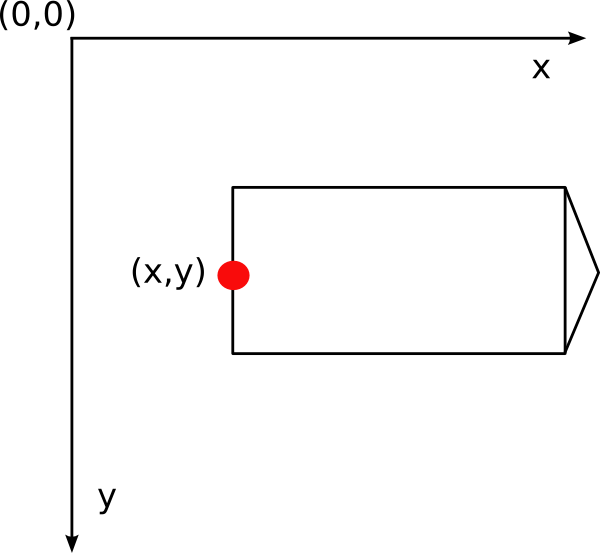
\includegraphics[width=7cm]{resources/img/repere.png}
\caption{Interpretation of the coordinates of boxes\label{fig-box-coordinates}}
\end{center}
\end{figure}

\bigskip
\noindent \textit{N} represents the number of outgoing transitions of the box.
This number is always $0$ for the final state.

\bigskip
\noindent The transitions are defined by the number of their target box.

\bigskip
\noindent Every line of the box definition ends with a newline.

\subsection{Format .fst2}
\index{File!\verbc{.fst2}}
An \verb+.fst2+ file is a text file that describes a set of graphs. Here is an
example of an \verb+.fst2+ file:

\bigskip
\verb+0000000002+\P

\verb+-1 NP+\P

\verb+: 1 1 +\P

\verb+: 2 2 -2 2 +\P

\verb+: 3 3 +\P

\verb+t +\P

\verb+f +\P

\verb+-2 Adj+\P

\verb+: 6 1 5 1 4 1 +\P

\verb+t +\P

\verb+f +\P

\verb+%<E>+\P

\verb+%the/DET+\P

\verb+%<A>/ADJ+\P

\verb+%<N>+\P

\verb+%nice+\P

\verb+@pretty+\P

\verb+%small+\P

\verb+f+\P

\bigskip
\noindent The first line represents the number of graphs that are encoded in the
file. The beginning of each graph is identified by a line that indicates the
number and the name of the graph (\verb+-1 NP+ and \verb+-2 Adj+ in the file
above).

\bigskip
\noindent The following lines describe the states of the graph. If the state is
final, the line starts with the \verb+t+ character and with the \verb+:+
character if not. For each state, the list of transitions is a possibly empty
sequence of pairs of integers:

\begin{itemize}
  \item the first integer indicates the number of the label or sub-graph that
  corresponds to the transition. Labels are numbered starting at 0. Sub-graphs
  are represented by negative integers, which explains why the numbers preceding
  the names of the graphs are negative;

  \item the second integer represents the number of the result state after the
  transition. In each graph, the states are numbered starting at 0. By convention
  state 0 is the initial state.

\end{itemize}

\bigskip
\noindent Each state definition line terminates with a space. The end of each
graph is marked by a line containing an \verb+f+ followed by a space and a
newline.

\bigskip
\noindent Labels are defined after the last graph. If the line begins with the
\verb+@+ character, the contents of the label is to be searched without allowing
case variations. This information is not used if the label is not a word. If the
line starts with a \verb+%+, capitalization variants are authorized. If a label
carries a transducer output sequence, the input and output sequences are
separated by the \verb+/+  character (example: \verb+the/DET+). By convention,
the first label is always the empty word (\verb+<E>+), even if that label is
never used for any transition.

\bigskip
\noindent The end of the file is indicated by a line containing the \verb+f+
character followed by a newline.



\section{Texts}
This section presents the different files used to represent texts.
\subsection{.txt files}
\index{File!\verbc{.txt}}\index{\verbt{\{S\}}}\index{Lexical!labels}
\index{Sentence delimiter}
\label{section-texts}
\verb+.txt+ files are text files encoded in Unicode Little-Endian. These files
should not contain any opening or closing braces, except for those used to mark a
sentence delimiter (\verb+{S}+) or a valid lexical tag
(\verb+{aujourd'hui,.ADV}+). The newline needs to be encoded with the two special
characters with hexadecimal values \verb+000D+ and \verb+000A+.


\subsection{.snt files}
\index{File!\verbc{.snt}}
\verb+.snt+ files are \verb+.txt+ files that have been processed by Unitex. These
files should not contain any tabs. They should also not contain multiple
consecutive spaces or newlines. The only allowed braces in \verb+.snt+ files are
those of the sentence delimiter \verb+{S}+\index{\verbt{\{S\}}}\index{Sentence
delimiter} and those of lexical labels
(\verb+{aujourd'hui,.ADV}+)\index{Lexical!labels}.


\subsection{File text.cod}
\index{File!\verbc{text.cod}}
The \verb+text.cod+ file is a binary file containing a sequence of integers that
represent the text. Each integer \verb+i+ reflects the token with index \verb+i+
in the \verb+tokens.txt+ file. These integers are encoded in four bytes.

\bigskip
\noindent NOTE: Tokens are numbered starting at 0.

\subsection{The tokens.txt file}
\index{File!\verbc{tokens.txt}}
The \verb+tokens.txt+ file is a text file that contains the list of all lexical
units of the text. The first line of this file indicates the number of units
found in the file. Units are separated by a newline. Whenever a sequence is found
in the text with capitalization variants, each variant is encoded as a distinct
unit.

\bigskip
\noindent NOTE: Newlines that might be in the \verb+.snt+ file are encoded like
spaces. Therefore there is no unit encoding the newline.

\subsection{The tok\_by\_alph.txt and tok\_by\_freq.txt files}
\index{File!\verbc{tok_by_alph.txt}}\index{File!\verbc{tok_by_freq.txt}}
These two files are text files that contain the list of lexical units sorted
alphabetically or by frequence.

\bigskip
\noindent In the \verb+tok_by_alph.txt+ file, each line is composed by a unit, followed by
a tab and the number of occurrences of the unit within the text.

\bigskip
\noindent The lines of the \verb+tok_by_freq.txt+ file are formed after the same principle,
but the number of occurrences is placed after the tab and the unit.


\subsection{The enter.pos file}
\index{File!\verbc{enter.pos}}
This file is a binary file containing the list of positions of the newline symbol
in the \verb+.snt+ file. Each position is the index in the \verb+text.cod+ file
where a newline has been replaced by a space. These positions are integers that
are encoded in 4 bytes.




\section{Text Automaton}

\subsection{The text.tfst file}
\label{section-tfst-format}
\index{File!\verbc{text.tfst}}
The \verb+text.tfst+ file represents the text automaton. It is a text
file that starts with a ten digit line indicating the number of sentence
automata it contains. Then, for each sentence automaton, you have the following
header lines:

\begin{itemize}
    \item \verb+$XXX+\P : \verb+XXX+ = number of the sentence

    \item \verb+foo foo foo...+\P : text of the sentence

    \item \verb+a/b c/d e/f g/h...+\P : for each token of the sentence, we
    have a pair \verb+x/y+: \verb+x+ is the token index in file
    \verb+tokens.txt+, \verb+y+ is the length of the token in characters

    \item \verb+X_Y+\P : \verb+X+ is the offset of the first token of the
    sentence, in tokens from the beginning of the text; \verb+Y+ is the same,
    but the offset is in characters from the beginning of the text.
\end{itemize}


\bigskip
\noindent Then, all states of the automaton are encoded, one per line. If the
state is final, the line starts with \verb+t+. Otherwise, the line starts with
\verb+:+. All transitions are written as pairs \verb+x y+, \verb+x+ being the
number of the tag, \verb+y+ being the number of the destination state. Note
that, at the opposite of \verb+.fst2+ format, lines have not to end with a
space. The and of state lines is marked by a line containing \verb+f+. 

\bigskip
\noindent Finally, all tags are encoded. By convention, the first tag is always
the epsilon one:

\bigskip
\noindent \verb$@<E>$\P

\noindent \verb$.$\P


\bigskip
\noindent Other labels have to be either lexical units or entries in the DELAF
format in braces. They are encoded as follows:

\bigskip
\noindent \verb$@STD$\P

\noindent \verb$@$\textit{content}\P

\noindent \verb$@$\textit{a}\verb$.$\textit{b}\verb$.$\textit{c}\verb$-$
\textit{x}\verb$.$\textit{y}\verb$.$\textit{z}\P

\noindent \verb$.$\P


\bigskip
\noindent \textit{content} is the tag content. The \textit{a.b.c-x.y.z}
information describe the zone in text covered by the tag:

\begin{itemize}
    \item \textit{a}: start offset in tokens from the beginning of the sentence;
    \item \textit{b}: start offset in characters from the beginning of the
    first token of the tag;
    \item \textit{c}: start offset in logical letters from the first character
    of the tag. This information is useful for Korean, because a tag can
    represent a Jamo sequence that occurs inside a Hangul character. Thus, the 
    character offset is not precise enough;\index{Jamo}\index{Hangul}
    \item \textit{x}: end offset in tokens from the beginning of the sentence;
    \item \textit{y}: end offset in characters from the beginning of the
    last token of the tag;
    \item \textit{z}: end offset in logical letters from the last character of
    the tag. In Korean sentence automata, empty surface forms can occur that
    correspond to the empty word in the text. In such cases, \textit{z} has
    special value $-1$.
\end{itemize}

\bigskip
\noindent The and of tag definitions is marked by a line containing \verb+f+.

\bigskip
\noindent Example: Here is the file that corresponds to the text \textit{He is
drinking orange juice.}

\bigskip
\noindent\verb$0000000001$\P

\noindent\verb+$1+\P

\noindent\verb$He is drinking orange juice. $\P

\noindent\verb$0/2 1/1 2/2 1/1 3/8 1/1 4/6 1/1 5/5 6/1 1/1$\P

\noindent\verb$0_0$\P

\noindent\verb$: 2 1 1 1$\P

\noindent\verb$: 4 2 3 2$\P

\noindent\verb$: 7 3 6 3 5 3$\P

\noindent\verb$: 10 5 9 4 8 4$\P

\noindent\verb$: 12 5 11 5$\P

\noindent\verb$: 13 6$\P

\noindent\verb$t$\P

\noindent\verb$f$\P

\noindent\verb$@<E>$\P

\noindent\verb$.$\P

\noindent\verb$@STD$\P

\noindent\verb$@{He,he.N:s:p}$\P

\noindent\verb$@0.0.0-0.1.0$\P

\noindent\verb$.$\P

\noindent\verb$@STD$\P

\noindent\verb$@{He,he.PRO+Nomin:3ms}$\P

\noindent\verb$@0.0.0-0.1.0$\P

\noindent\verb$.$\P

\noindent\verb$@STD$\P

\noindent\verb$@{is,be.V:P3s}$\P

\noindent\verb$@2.0.0-2.1.0$\P

\noindent\verb$.$\P

\noindent\verb$@STD$\P

\noindent\verb$@{is,i.N:p}$\P

\noindent\verb$@2.0.0-2.1.0$\P

\noindent\verb$.$\P

\noindent\verb$@STD$\P

\noindent\verb$@{drinking,drinking.A}$\P

\noindent\verb$@4.0.0-4.7.0$\P

\noindent\verb$.$\P

\noindent\verb$@STD$\P

\noindent\verb$@{drinking,drinking.N:s}$\P

\noindent\verb$@4.0.0-4.7.0$\P

\noindent\verb$.$\P

\noindent\verb$@STD$\P

\noindent\verb$@{drinking,drink.V:G}$\P

\noindent\verb$@4.0.0-4.7.0$\P

\noindent\verb$.$\P

\noindent\verb$@STD$\P

\noindent\verb$@{orange,orange.A}$\P

\noindent\verb$@6.0.0-6.5.0$\P

\noindent\verb$.$\P

\noindent\verb$@STD$\P

\noindent\verb$@{orange,orange.N:s}$\P

\noindent\verb$@6.0.0-6.5.0$\P

\noindent\verb$.$\P

\noindent\verb$@STD$\P

\noindent\verb$@{orange juice,orange juice.N+XN+z1:s}$\P

\noindent\verb$@6.0.0-8.4.0$\P

\noindent\verb$.$\P

\noindent\verb$@STD$\P

\noindent\verb$@{juice,juice.N+Conc:s}$\P

\noindent\verb$@8.0.0-8.4.0$\P

\noindent\verb$.$\P

\noindent\verb$@STD$\P

\noindent\verb$@{juice,juice.V:W:P1s:P2s:P1p:P2p:P3p}$\P

\noindent\verb$@8.0.0-8.4.0$\P

\noindent\verb$.$\P

\noindent\verb$@STD$\P

\noindent\verb$@.$\P

\noindent\verb$@9.0.0-9.0.0$\P

\noindent\verb$.$\P

\noindent\verb$f$\P






\subsection{The text.tind file}
\index{File!\verbc{text.tind}}
The \verb+text.tind+ file is an index file used to jump at correct byte offset
in the \verb+text.tfst+ file when we want to load a given sentence. It is a
binary file that contains $4 \times N$ bytes, where $N$ is the number of
sentences. It gives the start offset of each sentence as a 4-byte
little-endian sequence.


\subsection{The cursentence.grf file}
\label{section-cursentence_grf}
\index{File!\verbc{cursentence.grf}}
The \verb+cursentence.grf+ file is generated by Unitex during the display of a
sentence automaton. The \verb+Fst2Grf+ program constructs a \verb+.grf+ file from
the \verb+text.fst2+ file that represents a sentence automaton.

\bigskip
\noindent NOTE: outputs of graph boxes are used to encode offsets, as defined 
in \verb+.tfst+ tags. Offsets are separated with spaces. For instance, here are
some lines of the graph representing the first sentence of \textit{Ivanhoe}:

\bigskip
\noindent \verb$"Ivanhoe/0 0 0 0 6 0" 100 200 2 3 4 $\P
 
\noindent \verb$"{by,by.PART}/2 0 0 2 1 0" 220 150 2 5 6 $\P

\noindent \verb$"{by,by.PREP}/2 0 0 2 1 0" 220 50 2 5 6 $\P

\noindent \verb$"{Sir,sir.N+Hum:s}/4 0 0 4 2 0" 310 200 1 7$\P 




\subsection{The sentenceN.grf file}
Whenever the user modifies a sentence automaton, that automaton is saved under
the name \verb+sentenceN.grf+, where \verb+N+ represents the number of the
sentence. Such a graph contains offsets in graph box outputs (see note in
section \ref{section-cursentence_grf}).


\subsection{The cursentence.txt file}
\index{File!\verbc{cursentence.txt}}
During the extraction of the sentence automaton, the text of the sentence is
saved in the file called \verb+cursentence.txt+. That file is used by Unitex to
display the text of the sentence under the automaton. That file contains the text
of the sentence, followed by a newline.

\subsection{The cursentence.tok file}
\index{File!\verbc{cursentence.tok}}
During the extraction of the sentence automaton, the numbers of the tokens that
compose the sentence are stored in a file named \verb+cursentence.tok+. This
file contains one line per token, each line being made of 2 integers \verb$x y$:
\verb$x$ is the token number, \verb$y$ is the length of the token in characters.

\bigskip
\noindent Here is the content of this file for the first sentence of
\textit{Ivanhoe}:

\bigskip
\noindent \verb$0 7$\P \verb$         $\textit{Ivanhoe}

\noindent \verb$1 1$\P \verb$         $\texttt{\char `\ }

\noindent \verb$2 2$\P \verb$         $\textit{by}

\noindent \verb$1 1$\P \verb$         $\texttt{\char `\ }

\noindent \verb$3 3$\P \verb$         $\textit{Sir}

\noindent \verb$1 1$\P \verb$         $\texttt{\char `\ }

\noindent \verb$4 6$\P \verb$         $\textit{Walter}

\noindent \verb$1 1$\P \verb$         $\texttt{\char `\ }

\noindent \verb$5 5$\P \verb$         $\textit{Scott}

\noindent \verb$1 1$\P \verb$         $\texttt{\char `\ }


\subsection{The tfst\_tags\_by\_freq.txt and tfst\_tags\_by\_alph.txt files}
\index{File!\verbc{tfst_tags_by_freq.txt}}
\index{File!\verbc{tfst_tags_by_alph.txt}}
Those files contain all the tags that appear in the text automaton sorted by frequence and alphabetical order.


\section{Concordances}
\subsection{The concord.ind file}
\index{File!\verbc{concord.ind}}
The \verb+concord.ind+ file is the index of the occurrences found by either
\verb+Locate+ or \verb+LocateTfst+ during the application of a grammar. It is a
text file that contains the starting and ending positions of each occurrence,
possibly accompanied by a sequence of letters if the construction of the concordance took
into account the possible transducer outputs of the grammar. 
Here is an example
of such a file:

\bigskip
\verb$#M$\P

\verb$59.0.0 63.3.0 the[ADJ= greater] part$\P

\verb$67.0.0 71.4.0 the beautiful hills$\P

\verb$87.0.0 91.3.0 the pleasant town$\P

\verb$123.0.0 127.4.0 the noble seats$\P

\verb$157.0.0 161.5.0 the fabulous Dragon$\P

\verb$189.0.0 193.3.0 the Civil Wars$\P

\verb$455.0.0 459.11.0 the feeble interference$\P

\verb$463.0.0 467.6.0 the English Council$\P

\verb$566.0.0 570.10.0 the national convulsions$\P

\verb$590.0.0 594.5.0 the inferior gentry$\P

\verb$626.0.0 630.11.0 the English constitution$\P

\verb$696.0.0 700.4.0 the petty kings$\P

\verb$813.0.0 817.5.0 the certain hazard$\P

\verb$896.0.0 900.5.0 the great Barons$\P

\verb$938.0.0 942.3.0 the very edge$\P

\bigskip
\noindent The first line indicates in which transduction mode the concordance has
been constructed. The three possible values are:

\begin{itemize}
  \item \verb+#I+ : transducer outputs have been ignored;

  \item \verb+#M+ : transducer outputs have been inserted before the
  corresponding inputs (MERGE mode);
  \index{MERGE}
  
  \item \verb+#R+ : transducer outputs have replaced the recognized sequences (REPLACE mode)).
  \index{REPLACE}
\end{itemize}

\bigskip
\noindent Each occurrence is described in one line. The lines start with the start
and end positions of the occurrence. These positions corresponds to the offsets
defined in \verb$.tfst$ tags (see \ref{section-tfst-format}).

\bigskip
\noindent If the file has the heading line \verb+#I+, the end position of each
occurrence is immediately followed by a newline. Otherwise, it is followed by a
space and a sequence of characters. In REPLACE mode, that sequence corresponds to
the output produced for the recognized sequence. In MERGE mode, it represents the
recognized sequences into which the outputs have been inserted. In MERGE or
REPLACE mode, this sequence is displayed in the concordance. If the outputs have
been ignored, the contents of the occurrence is extracted from the text file.


\subsection{The concord.txt file}
\index{File!\verbc{concord.txt}}
The \verb+concord.txt+ file is a text file that represents a concordance. Each
occurrence is encoded in a line that is composed of three character sequences
separated by a tab, representing the left context, the occurrence (possibly
modified by transducer outputs) and the right context.


\subsection{The concord.html file}
\index{File!\verbc{concord.html}}
The \verb+concord.html+ file is an \verb+HTML+ file that represents a
concordance. This file is encoded in UTF-8.\index{UTF-8}

\bigskip
\noindent The title of the page is the number of occurrences it describes. The
lines of the concordance are encoded as lines where the occurrences are
considered to be hypertext lines. The reference associated to each of these lines
has the following form: \verb+<a href="X Y Z">+. \verb+X+ and \verb+Y+ represent
the start and end position of the occurrence in characters in the file
\verb+name_of_text.snt+. \verb+Z+ represents the number of the phrase in which
this occurrence appears.

\bigskip
\noindent All spaces that are at the left and right edges of lines are encoded by
a non breaking space (\verb+&nbsp;+ in HTML), which allows the preservation of
the alignment of the occurrences even if one of them has a left context with
spaces.

\bigskip
\noindent NOTE: If the concordance has been constructed with the \verb+glossanet+
parameter, the HTML file has the same structure, except for the links. In
these concordances, the occurrences are real links pointing at the web server of
the GlossaNet application. For more information on GlossaNet, consult the link on
the Unitex web site. \index{GlossaNet}

\bigskip
\noindent Here is an example of a file:

\bigskip

\verb$<html lang=en>$\P

\verb$<head>$\P

\verb$$\P

\verb$   <meta http-equiv="Content-Type" content="text/html;$

\verb$         charset=UTF-8">$\P

\verb$   <title>6 matches</title>$\P

\verb$</head>$\P

\verb$<body>$\P

\verb$<table border="0" cellpadding="0" width="100%" $

\verb$       style="font-family: 'Arial Unicode MS'; font-size: 12">$\P

\verb$<font face="Courier new" size=3>$\P

\verb$on, there <a href="116 124 2">extended</a>&nbsp;i&nbsp;<br>$\P

\verb$&nbsp;extended <a href="125 127 2">in</a>&nbsp;ancient&nbsp;<br>$\P

\verb$&nbsp;Scott {S}<a href="32 34 2">IN</a>&nbsp;THAT PL&nbsp;<br>$\P

\verb$STRICT of <a href="61 66 2">merry</a>&nbsp;Engl&nbsp;<br>$\P

\verb+S}IN THAT <a href="40 48 2">PLEASANT</a>&nbsp;D&nbsp;<br>+\P

\verb+&nbsp;which is <a href="84 91 2">watered</a>&nbsp;by&nbsp;<br>+\P

\verb$</font>$\P

\verb$</td></table></body>$\P

\verb$</html>$\P


\bigskip
\noindent Figure \ref{fig-example-concordance-2} shows the page that
corresponds to the file below.

\begin{figure}[!ht]
\begin{center}
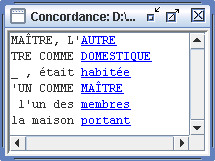
\includegraphics[width=5cm]{resources/img/fig10-2.png}
\caption{Example of a concordance\label{fig-example-concordance-2}}
\end{center}
\end{figure}



\subsection{The diff.html file}
\index{File!\verbc{diff.html}}
The \verb+diff.html+ file is an \verb+HTML+ file that presents the differences
between two concordances. This file is encoded in UTF-8.\index{UTF-8} Here is an
example of file (new lines have been introduced for presentation convenience):


\begin{verbatim}
<html>
<head>
<meta http-equiv="Content-Type" content="text/html;
charset=UTF-8">
<style type="text/css">
a.blue {color:blue; text-decoration:underline;}
a.red {color:red; text-decoration:underline;}
a.green {color:green; text-decoration:underline;}
</style>
</head>
<body>
<h4>
<font color="blue">Blue:</font> identical sequences<br>
<font color="red">Red:</font> similar but different sequences<br>
<font color="green">Green:</font> sequences that occur in only
one of the two concordances<br>
<table border="1" cellpadding="0" style="font-family: Courier new;
font-size: 12">
<tr><td width="450"><font color="blue">ed in ancient times
<u>a large forest</u>, covering the greater par</font></td>
<td width="450"><font color="blue">ed in ancient times
<u>a largeforest</u>, covering the greater par</font></td>
</tr>
<tr><td width="450"><font color="green">ge forest, covering
<u>the greater part</u>&nbsp;of the beautiful hills </font>
</td>
<td width="450"><font color="green"></font></td>
</tr>
</table>
</body>
</html>
\end{verbatim}


\section{Text dictionaries}
The \verb+Dico+ program produces several files that represent text dictionaries.

\subsection{dlf and dlc}
\index{File!\verbc{dlf}}
\index{File!\verbc{dlc}}

\verb+dlf+ and \verb+dlc+ are simple and compound word dictionaries in the DELAF
format (see section \ref{section-DELAF-format}).

\subsection{err}
\index{File!\verbc{err}}
This file is made of unkown words, one per line.

\subsection{tags\_err}
\index{File!\verbc{tags_err}}
This file is made of unkown words, one per line. The difference with the \verb+err+ file is that 
in this one do not appear simple words that have been matched in the \verb+tags.ind+ file.

\subsection{tags.ind}
\index{File!\verbc{tags.ind}}
\label{section-tags-ind}
This file has the same format than a \verb+concord.ind+ one obtained in MERGE
or REPLACE mode, but its header is \verb+#T+. Note that the outputs DO NOT BEGIN
with a slash.
 


\section{Dictionaries}
The compression of the DELAF dictionaries by the \verb+Compress+ program produces
two files: a \verb+.bin+ file that represents the minimal automaton of the
inflected forms of the dictionaries, and a \verb+.inf+ file that contains the
compressed forms required for the construction of the dictionaries from the
inflected forms. This section describes the format of these two file types, as
well as the format of the \verb+CHECK_DIC.TXT+ file, which contains the result of
the verification of a dictionary.
\index{\verbc{Compress}}\index{External programs!\verbc{Compress}}

\index{DELAF}\index{Dictionaries!DELAF}

\subsection{The .bin files}
\index{File!\verbc{.bin}}
A \verb$.bin$ file is a binary file that represents an automaton. The first 4
bytes of the file represent an integer that indicates the size of the file in
bytes. The states of the automaton are encoded in the following way:
\begin{itemize}

  \item the first two bytes indicate if the state is final as well as the number
  of its outgoing transitions. The highest bit is 0 if the state is final, 1 if
  not. The other 15 bits encode the number of transitions.

  \bigskip Example: a non-final state with 17 transitions is encoded by the
  hexadecimal sequence 8011
  

  \bigskip \item if the state is final, the three following bytes encode the
  index in the \verb+.inf+ file of the compressed form to be used to reconstruct
  the dictionary lines for this inflected form.

  
  \bigskip Example: if the state refers to the compressed form with index 25133,
  the corresponding hexadecimal sequence is \verb+00622D+
  

  \bigskip \item each leaving transition is then encoded in 5 bytes. The first 2
  bytes encode the character that labels the transition, and the three following
  encode the byte position of the result state in the \verb+.bin+ file. The
  transitions of a state are encoded next to each other.

  \bigskip Example: a transition that is labeled with the \verb+A+ letter and
  goes to the state of which the description starts at byte 50106, is represented
  by the hexadecimal sequence \verb+004100C3BA+.

\end{itemize}

\bigskip
\noindent By convention, the first state of the automaton is the initial state.

\subsection{The .inf files}
\index{File!\verbc{.inf}}
A \verb+.inf+ file is a text file that describes the compressed files that are
associated to a \verb+.bin+ file. Here an example of a \verb+.inf+ file:

\bigskip
\verb$0000000006$\P

\verb$_10\0\0\7.N$\P

\verb$.PREP$\P

\verb$_3.PREP$\P

\verb$.PREP,_3.PREP$\P

\verb$1-1.N+Hum:mp$\P

\verb$3er 1.N+AN+Hum:fs$\P

\bigskip
\noindent The first line of the file indicates the number of compressed forms that
it contains. Each line can contain one or more compressed forms. If there are
multiple forms, they are separated by commas. Each compressed form is made up of
a sequence required to reconstruct a canonical knowing an inflected form,
followed by a sequence of grammatical, semantic and inflection codes that are
associated to the entry.

\bigskip
\noindent The mode of compression of the canonical form varies in function of the
inflected form. If the two forms are identical, the compressed form contains only
the grammatical, semantic and inflectional information as in:

\bigskip
\verb$.N+Hum:ms$

\bigskip
\noindent If the forms are different, the compression program cuts up the two
forms in units. These units can be a space, a hyphen, or a sequence of characters
that contains neither a space nor a hyphen. This way of cutting up units allows
the program to efficiently take into account the inflected forms of the compound
words.

\bigskip
\noindent If the inflected and the canonical form do not have the same number of
units, the program encodes the canonical form by the number of characters to be
removed from the inflected form followed by the characters to append. For
instance, the line below is a line in the initial dictionary:

\bigskip
\verb+James Bond,007.N+

\bigskip
\noindent Since the sequence \verb+James Bond+ contains three units and \verb+007+ only
one, the canonical form is encoded with \verb+_10\0\0\7+. The \verb+_+ character
indicates that the two forms do not have the same number of units. The following
number (here 10) indicates the number of characters to be removed. The sequence
\verb+\0\0\7+ indicates that the sequence \verb+007+ should be appended. The
digits are preceeded by the \verb+\+ character so they will not be confused with
the number of characters to be removed.

\bigskip
\noindent Whenever the two forms have the same number of units, the units are compressed
two by two. Each pair consists of a unit the inflected form and the corresponding
unit in the canonical form. If each of the two units is a space or a hyphen, the
compressed form of the unit is the unit itself, as in the following line:


\bigskip
\verb$0-1.N:p$

\bigskip
\noindent which is the output for \verb$battle-axes,battle-axe.N:p$

\bigskip
\noindent This maintains a certain readability of the \verb+.inf+ file when the dictionary
contains compound words.

\bigskip
\noindent Whenever one or both of the units in a pair is neither a space nor a
hyphen, the compressed form is composed of the number of characters to be removed
followed by the sequence of characters to be appended. Thus, the dictionary line:

\bigskip
\noindent
\texttt{premi\`ere partie,premier parti.N+AN+Hum:fs}

\bigskip
\noindent is encoded by the line:

\bigskip
\verb$3er 1.N+AN+Hum:fs$

\bigskip
\noindent The \verb+3er+ code indicates that 3 characters are to be removed from
the sequence \texttt{premi\`ere} and the characters \verb+er+ are to be appended
to obtain \verb+premier+. The \verb+1+ indicates that only one character needs to be
removed from \verb+partie+ to obtain \verb+parti+. The number \verb+0+ is used
whenever it needs to be indicated that no letter should be removed.


\subsection{Dictionary information file}
\index{Dictionary information file}
In the "Apply lexical resources" frame, it is possible for some dictionaries to
get some information with a right click. Such information is attached to a
\verb+biniou.bin+ or \verb+biniou.fst2+ dictionary by the mean of a raw text
file named \verb+biniou.txt+, located in the same directory.

\subsection{The CHECK\_DIC.TXT file}
\index{File!\verbc{CHECK_DIC.TXT}}\index{\verbc{CheckDic}}\index{External programs!\verbc{CheckDic}}
This file is produced by the dictionary verification program \verb+CheckDic+. It
is a text file that contains information about the analysed dictionary and has
four parts.

\bigskip
\noindent The first part is the possibly empty list of all syntax errors found in
the dictionary: absence of the inflected or the canonical form, the grammatical
code, empty lines, etc. Each error is described by the number of the line, a
message describing the error, and the contents of the line. Here is an example
of a message:

\begin{verbatim}
Line 12451: unexpected end of line
garden,N:s
\end{verbatim}

\bigskip
\noindent The second and third parts display the list of grammatical codes and/or semantic
and inflectional codes respectively. In order to prevent coding errors, the
program reports encodings that contain spaces, tabs, or non-ASCII characters. For
instance, if a Greek dictionary contains the \verb+ADV+ code where the Greek
\verb+A+ character is used instead of the Latin \verb+A+ character, the program
reports the following warning:

\begin{verbatim}
ADV warning: 1 suspect char (1 non ASCII char): (0391 D V)
\end{verbatim}

\bigskip
\noindent Non-ASCII characters are indicated by their hexadecimal character number. In the
example below, the code \verb+0391+ represents Greek \verb+A+. Spaces are
indicated by the \verb+SPACE+ sequence:

\begin{verbatim}
Km s warning: 1 suspect char (1 space): (K m SPACE s)
\end{verbatim}

\bigskip
\noindent When the following dictionary is checked:

\begin{verbatim}
1,2 et 3!,.INTJ 
abracadabra,INTJ 
supercalifragilisticexpialidocious,.INTJ
damned,. INTJ
Paul,.N+Hum+Hum
eat,.V:W:P1s:Ps:P1p:P2p:P3p
\end{verbatim}

\bigskip
\noindent the following \verb+CHECK_DIC.TXT+ file is obtained:

\bigskip
\verb$Line 1: unprotected comma in lemma$\P

\verb$1,2 et 3!,.INTJ $\P

\verb$Line 2: unexpected end of line$\P

\verb$abracadabra,INTJ $\P

\verb$Line 5: duplicate semantic code$\P

\verb$Paul,.N+Hum+Hum$\P

\verb$Line 6: an inflectional code is a subset of another$\P

\verb$eat,.V:W:P1s:Ps:P1p:P2p:P3p$\P

\verb$-----------------------------------$\P

\verb$-------------  Stats  -------------$\P

\verb$-----------------------------------$\P

\verb$File: D:\My Unitex\English\Dela\axe.dic$\P

\verb$Type: DELAF$\P

\verb$6 lines read$\P

\verb$2 simple entries for 2 distinct lemmas$\P

\verb$0 compound entry for 0 distinct lemma$\P

\verb$-----------------------------------$\P

\verb$----  All chars used in forms  ----$\P

\verb$-----------------------------------$\P

\verb$a (0061)$\P

\verb$c (0063)$\P

\verb$d (0064)$\P

\verb$e (0065)$\P

\verb$f (0066)$\P

\verb$g (0067)$\P

\verb$i (0069)$\P

\verb$l (006C)$\P

\verb$m (006D)$\P

\verb$n (006E)$\P

\verb$o (006F)$\P

\verb$p (0070)$\P

\verb$r (0072)$\P

\verb$s (0073)$\P

\verb$t (0074)$\P

\verb$u (0075)$\P

\verb$x (0078)$\P

\verb$-------------------------------------------------------------$\P

\verb$----    2 grammatical/semantic codes used in dictionary  ----$\P

\verb$-------------------------------------------------------------$\P

\verb$INTJ$\P

\verb$ INTJ warning: 1 suspect char (1 space): (SPACE I N T J)$\P

\verb$-----------------------------------------------------$\P

\verb$----    0 inflectional code used in dictionary  -----$\P

\verb$-----------------------------------------------------$\P

\bigskip
\noindent Note that the inflectional codes of \verb+eat+ are not reported, since
an error occurred in this line.


\section{ELAG files}
\subsection{tagset.def file}
\index{File!\verbc{tagset.def}}
See section \ref{section-elag-tagset}, page \pageref{section-elag-tagset}.

\subsection{.lst files}
\index{File!\verbc{.lst}}

.LST FILES ARE NOT UNICODE FILES.

\bigskip
\noindent A \verb$.lst$ file contains a list of \verb$.grf$ file names. If
a file's path is not absolute, it is relative to the location
of the \verb$elag.lst$ file. Here is the \verb$elag.lst$ file used for French:


\bigskip
\verb$PPVs/PpvIL.grf$\P

\verb$PPVs/PpvLE.grf$\P

\verb$PPVs/PpvLUI.grf$\P

\verb$PPVs/PpvPR.grf$\P

\verb$PPVs/PpvSeq.grf$\P

\verb$PPVs/SE.grf$\P

\verb$PPVs/postpos.grf$\P

\subsection{.elg files}
\index{File!\verbc{.elg}}

\verb$.elg$ files contain compiled ELAG rules. These files are in the
\verb$.fst2$ format.


\subsection{.rul files}
\index{File!\verbc{.rul}}

.RUL FILES ARE NOT UNICODE FILES.

\bigskip
\noindent A \verb$.rul$ file contains the different \verb$.elg$ files that compose an ELAG
rule set. It contains one part per \verb$.elg$ file. Each part lists the ELAG
grammars that correspond to a given \verb$.elg$ file. \verb$.elg$ file names are
surrounded with angles brackets. The lines that start with a tabulation are
considered as comments by the \verb+Elag+
program.\index{\verbc{Elag}}\index{External programs!\verbc{Elag}} Here is the
\verb$elag.rul$ file used for French:

\bigskip
\verb$    PPVs/PpvIL.elg$\P

\verb$    PPVs/PpvLE.elg$\P

\verb$    PPVs/PpvLUI.elg$\P

\verb$<elag.rul-0.elg>$\P

\verb$    PPVs/PpvPR.elg$\P

\verb$    PPVs/PpvSeq.elg$\P

\verb$    PPVs/SE.elg$\P

\verb$    PPVs/postpos.elg$\P

\verb$<elag.rul-1.elg>$\P

\section{Tagger files}
This section presents files produced and used by TrainingTagger and Tagger programs.

\subsection{The corpus.txt file}
\index{File!\verbc{corpus.txt}}
\label{section-corpus-file}
This file is used by the TrainingTagger program in order to compute statistics for the Tagger program. It contains sentences 
where each word is represented in a separate line. Each line representing a word is composed of a word, simple or compound, 
followed by a slash and the tag of the word. This tag is composed of a grammatical code, sometimes followed by a \verb$'+'$ and 
syntactic or semantic codes. Inflectional codes are specified after a \verb+':'+. If the word is a compound, simple words contained 
in it must be separated by a \verb+'_'+. 
Here is an example of a corpus.txt file :

\bigskip
\verb$The/DET+Ddef:s$\P

\verb+GATT/N:s+\P

\verb+had/V:I3s+\P

\verb+formerly/ADV+\P

\verb$a/DET+Dind:s$\P

\verb+political/A+\P

\verb+assessment/N:s+\P

\verb+of/PREP+\P

\verb$the/DET+Ddef:s$\P

\verb+behavior/N:s+\P

\verb+of/PREP+\P

\verb+foreign_countries/N:p+\P

\verb+./PONCT+\P

\P

\verb$She/PRO+Nomin:3fs$\P

\verb+closed/V:I3s+\P

\verb+easily/ADV+\P

\verb$her/DET+Poss3fs:p$\P

\verb+eyes/N:p+\P

\verb+when/CONJ+\P

\verb$some/DET+Dadj:p$\P

\verb+infractions/N:p+\P

\verb+might/V:I3p+\P

\verb+appear/V:W+\P

\verb+justified/V:K+\P

\verb+against/PREP+\P

\verb+higher/A+\P

\verb+interests/N:p+\P

\verb+./PONCT+\P

\P

\bigskip
\noindent NOTE: Sentences must be delimited by empty lines.

\bigskip
The \verb+.txt+ file format can also be used (see section \ref{section-texts}). Each word of the text 
must be represented by a valid lexical label (\verb+{aujourd'hui,.ADV}+)\index{Lexical!labels} and sentences
are delimited by  \verb+{S}+\index{\verbt{\{S\}}}\index{Sentence delimiter}.
Here is the previous example in the \verb+.txt+ file format :

\bigskip
\verb${The,.DET+Ddef:s}$ \verb${GATT,.N:s}$ \verb${had,.V:I3s}$ \verb${formerly,.ADV}$\\ 
\verb${a,.DET+Dind:s}$ \verb${political,.A}$ \verb${assessment,.N:s}$ \verb${of,.PREP}$\\ 
\verb${the,.DET+Ddef:s}$ \verb${behavior,.N:s}$ \verb${of,.PREP}$ \verb${foreign countries,.N:p}$\\ 
\verb${.,.PONCT}$ \verb${S}$ \verb${She,.PRO+Nomin:3fs}$ \verb${closed,.V:I3s}$ \verb${easily,.ADV}$\\
\verb${her,.DET+Poss3fs:p}$ \verb${eyes,.N:p}$ \verb${when,.CONJ}$ \verb${some,.DET+Dadj:p}$\\
\verb${infraction,.N:p}$ \verb${might,.V:I3p}$ \verb${appear,.V:W}$ \verb${justified,.V:K}$\\
\verb${against,.PREP}$ \verb${higher,.A}$ \verb${interests,.N:p}$ \verb${.,.PONCT}$ \verb${S}$

\subsection{The tagger data file}
\index{File!\verbc{train_dict}}
\label{section-training-dict}
The TrainingTagger program generates two data files (by default) used by the Tagger program in order
to compute a second-order hidden Markov model. 
These files contain unigram, bigram and trigram tuples extracted from the tagged corpus.txt file. Tuples are
composed of either a sequence of 2 or 3 tags (to compute transition probability) or a word preceded by
0 or 1 tag (to compute emit probability). Units in a tuple must be separated by a tabulation.
These tuples are followed by the sequence of delimiters ",." and then an integer representing the number of
occurrences of this tuple in the corpus file. 

\bigskip
\noindent Filenames are suffixed by "cat" or "morph". In the first one, tuples are composed of tags formed of grammatical, 
syntactic and semantic codes. In the second one, tuples consist in tags formed of grammatical, syntactic and semantic 
codes and sometimes followed by a \verb+':'+ and inflectional codes.
Here is an example of a data file with "cat" tags : 

\bigskip
\verb+the,.9630+\P

\verb+those,.236+\P

\verb+eyes,.32+\P

\verb$DET+Ddef	 the,.9630$\P

\verb$DET+Ddem	 those,.140$\P

\verb$PRO+Pdem	 those,.96$\P

\verb+N		   eyes,.32+\P

\verb+DET	 N,.62541+\P

\verb+PREP	DET  N,.25837+\P

\P

\bigskip

\noindent Here is an example of a data file with "morph" tags :

\bigskip
\verb+the,.9630+\P

\verb+those,.236+\P

\verb+eyes,.32+\P

\verb$DET+Ddef:s	 the,.4437$\P

\verb$DET+Ddef:p	 the,.5193$\P

\verb$DET+Ddem:p	 those,.140$\P

\verb$PRO+Pdem:p	 those,.96$\P

\verb+N:p		   eyes,.32+\P

\verb+DET:s	 N:s,.18489+\P

\verb+PREP	  DET:s  N:s,.6977+\P

\P

\bigskip
\noindent A special line is added to data files in order to identify whether the file contains "cat" or "morph" tags. 
This line contains \verb+CODE FEATURES+ followed by either the integer 0 for "cat" tags or 1 for
"morph" tags.

\bigskip
\noindent NOTE: At the final stage, TrainingTagger compresses these two data files into the ".bin" format.


\section{Configuration files}
\subsection{The Config file}
\index{File!\verbc{Config}}
Whenever the user modifies his preferences for a given languages, these
modifications are saved in a text file named 'Config' which can be found in the
directory of the current language. The file has the following syntax (the order
of lines can vary):


\bigskip
\verb$#Unitex configuration file of 'paumier' for 'English'$\P

\verb$#Fri Oct 10 15:18:06 CEST 2008$\P

\verb$TEXT\ FONT\ NAME=Courier New$\P

\verb$TEXT\ FONT\ STYLE=0$\P

\verb$TEXT\ FONT\ SIZE=10$\P

\verb$CONCORDANCE\ FONT\ NAME=Courier new$\P

\verb$CONCORDANCE\ FONT\ HTML\ SIZE=12$\P

\verb$INPUT\ FONT\ NAME=Times New Roman$\P

\verb$INPUT\ FONT\ STYLE=0$\P

\verb$INPUT\ FONT\ SIZE=10$\P

\verb$OUTPUT\ FONT\ NAME=Arial Unicode MS$\P

\verb$OUTPUT\ FONT\ STYLE=1$\P

\verb$OUTPUT\ FONT\ SIZE=12$\P

\verb$DATE=true$\P

\verb$FILE\ NAME=true$\P

\verb$PATH\ NAME=false$\P

\verb$FRAME=true$\P

\verb$RIGHT\ TO\ LEFT=false$\P

\verb$BACKGROUND\ COLOR=-1$\P

\verb$FOREGROUND\ COLOR=-16777216$\P

\verb$AUXILIARY\ NODES\ COLOR=-3289651$\P

\verb$COMMENT\ NODES\ COLOR=-65536$\P

\verb$SELECTED\ NODES\ COLOR=-16776961$\P

\verb$PACKAGE\ NODES\ COLOR=-2302976$\P

\verb$CONTEXT\ NODES\ COLOR=-16711936$\P

\verb$CHAR\ BY\ CHAR=false$\P

\verb$ANTIALIASING=false$\P

\verb$HTML\ VIEWER=$\P

\verb$MAX\ TEXT\ FILE\ SIZE=2097152$\P

\verb$ICON\ BAR\ POSITION=West$\P

\verb$PACKAGE\ PATH=D\:\\repository$\P

\verb$MORPHOLOGICAL\ DICTIONARY=D\:\\MyUnitex\\English\\Dela\\zz.bin$\P

\verb$MORPHOLOGICAL\ NODES\ COLOR=-3911728$\P

\verb$MORPHOLOGICAL\ USE\ OF\ SPACE=false$\P


\bigskip
\noindent The first two lines are comment lines. The following three lines indicate the
name, the style and the size of the font used to display texts, dictionaries,
lexical units, sentences in text automata, etc.


\bigskip
\noindent The \verb$CONCORDANCE FONT NAME$ and \verb$CONCORDANCE FONT HTML SIZE$ parameters
define the name, the size and the font to be used when displaying concordances in
HTML. The size of the font has a value between 1 and 7.


\bigskip
\noindent The \verb$INPUT FONT ...$ and \verb$OUTPUT FONT ...$ parameters define the name,
the style and the size of the fonts used for displaying the paths and the
transducer outputs of the graphs.


\bigskip
\noindent The following 10 parameters correspond to the parameters given in the headings of
the graphs. Table \ref{tab-parameters} describes the
correspondances.

\begin{table}[!ht]
\begin{center}
\begin{tabular}{|c|c|}
\hline
Parameters in the \verb+Config+ file &  Parameters in the \verb+.grf+ file
\\
\hline
\verb$DATE$ & \verb$DDATE$
\\
\hline
\verb$FILE NAME$ & \verb$DFILE$
\\
\hline
\verb$PATH NAME$ & \verb$DDIR$
\\
\hline
\verb$FRAME$ & \verb$DFRAME$
\\
\hline
\verb$RIGHT TO LEFT$ & \verb$DRIG$
\\
\hline
\verb$BACKGROUND COLOR$ & \verb$BCOLOR$
\\
\hline
\verb$FOREGROUND COLOR$ & \verb$FCOLOR$
\\
\hline
\verb$AUXILIARY NODES COLOR$ & \verb$ACOLOR$
\\
\hline
\verb$COMMENT NODES COLOR$ & \verb$SCOLOR$
\\
\hline
\verb$SELECTED NODES COLOR$ & \verb$CCOLOR$
\\
\hline
\end{tabular}
\caption{Meaning of the parameters\label{tab-parameters}}
\end{center}
\end{table}

\bigskip
\noindent The \verb+PACKAGE NODES+ parameter defines the color to be used for
displaying calls to subgraphs located in the repository.

\bigskip
\noindent The \verb+CONTEXT NODES+ parameter defines the color to be used for
displaying boxes that correspond to context bounds.

\bigskip
\noindent The \verb+CONTEXT NODES+ indicates if the current language must be
tokenized character by character or not.

\bigskip
\noindent The \verb+ANTIALIASING+ parameter indicates whether graphs as well as
sentence automata are displayed by default with the antialiasing effect.
\index{Antialiasing}

\bigskip
\noindent The \verb+HTML VIEWER+ parameter indicates the name of the navigator to
be used for displaying concordances. If no navigator name is defined,
concordances are displayed in a Unitex window.

\bigskip
\noindent The \verb+MAX TEXT FILE SIZE+ parameter is deprecated.

\bigskip
\noindent The \verb+ICON BAR POSITION+ parameter indicates the default position of
icon bars in graph frames.

\bigskip
\noindent The \verb+PACKAGE PATH+ parameter specifies the location of the
repository.

\bigskip
\noindent The \verb+MORPHOLOGICAL DICTIONARY+ parameter specifies the list of
morphological-mode dictionaries, separated with semi-colons.

\bigskip
\noindent The \verb+MORPHOLOGICAL NODES COLOR+ parameter specifies the color
to use to render the \verb+$<+ and \verb+$>+ tags. 

\bigskip
\noindent The \verb+MORPHOLOGICAL USE OF SPACE+ parameter indicates if the
\verb+Locate+ program is allowed to start matching on spaces. Default is false. 


\subsection{The system\_dic.def file}
\index{File!\verbc{system_dic.def}}
The \verb+system_dic.def+ file is a text file that describes the list of system
dictionaries that are applied by default. This file can be found in the directory
of the current language. Each line corresponds to a name of a .bin file. The
system dictionaries are in the Unitex system directory,\index{Directory!Unitex system}
and within that directory, in the
\verb+(current language)/Dela+ sub-directory. \index{File!\verbc{.bin}} Here is an
example of this file:


\bigskip
\verb$delacf.bin$\P

\verb$delaf.bin$\P

\subsection{The user\_dic.def file}
\index{File!\verbc{user_dic.def}}
The \verb+user_dic.def+ file is a text file that describes the list of
dictionaries the user has defined to be applied by default. This file is in the
directory of the current language and has the same format as the
\verb+system_dic.def+ file. 
The dictionaries need to be in the \verb+(current language)/Dela+ sub-directory of the
user's working directory.\index{Directory!personal working}

\subsection{The (user login).cfg and .unitex.cfg files}
\index{File!\verbc{.cfg}}
Under Linux and Mac OS, your working directory is expected to be called
\verb+unitex+ and to be in your root directory (\verb+$HOME+). If you want
to change this default location, a \verb+.unitex.cfg+ file is created in your home directory, and
it contains the path to your working directory. This file is a UTF8 one. If \verb+.unitex.cfg+
does not contain a valid Linux path to an existing directory, it is ignored.\,\footnote{This allows you
to launch Unitex sometimes under Linux, sometimes under Windows, on shared files: the Windows path to your
working directory is contained in \texttt{.unitex.cfg}, and Unitex ignores it when launched
under Linux.}

\bigskip
\noindent Under Windows, it is not always possible to associate a directory to a user by
default. To compensate for that, Unitex creates for each user a \verb+.cfg+ file
that contains the path to his/her working directory.\index{Directory!personal working}
This file is saved under the name \verb+(user login).cfg+ in the \verb+Users+ sub-directory
of the Unitex system directory.\index{Directory!Unitex system}
If the user does not have permission to write into this directory, Unitex saves a file named \verb+.unitex.cfg+
 in the Windows user profile directory:
\begin{itemize}
\item in \verb+Documents and Settings\(user login)+ if under Windows XP
\item in \verb+Users\(user login)+ if under WindowsVista or later.
\end{itemize}

\bigskip
\noindent WARNING:  THIS FILE IS NOT IN UNICODE

\bigskip
\noindent WARNING (2): THE PATH OF THE PERSONAL WORKING
DIRECTORY IS NOT FOLLOWED BY A NEWLINE.

\section{Cassys files}

\subsection{Cassys configuration files csc}

To memorize the list of transducer of a CasSys cascade, we use a text file (csc file) in which each line contains the path to a transducer followed by the output policy (merge/replace) to be applied to this transducer.
The generic format of a line of csc file is : Name\_and\_path\_of\_transducer  Merge
Here is an example of cascade file csc:

\ttfamily
"C:$\backslash$apps$\backslash$my\_unitex$\backslash$French$\backslash$Graphs$\backslash$grf1.fst2" Merge

"C:$\backslash$apps$\backslash$my\_unitex$\backslash$French$\backslash$Graphs$\backslash$grf2.fst2" Replace
\rmfamily

\section{Various other files}
For each text, Unitex creates multiple files that contain information that are
designed to be displayed in the graphical interface. This section describes these
files and some others.


\subsection{The dlf.n, dlc.n, err.n et tags\_err.n files}
\index{File!\verbc{dlf.n}}\index{File!\verbc{dlc.n}}\index{File!\verbc{err.n}}\index{File!\verbc{tags_err.n}}
\index{File!\verbc{dlf}}\index{File!\verbc{dlc}}\index{File!\verbc{err}}\index{File!\verbc{tags_err}}
These files are text files that are stored in the text directory. They
contain the number of lines of the \verb+dlf+, \verb+dlc+, \verb+err+ and \verb+tags_err+ files
respectively. These numbers are followed by a newline.


\subsection{The stat\_dic.n file}
\index{File!\verbc{stat_dic.n}}
This file is a text file in the directory of the text. It has three lines that
contain the number of lines of the \verb+dlf+, \verb+dlc+ and \verb+err+ files.

\subsection{The stats.n file}
\index{File!\verbc{stats.n}}
This file is in the text directory and contains a line with the following form:


\bigskip
\verb$3949 sentence delimiters, 169394 (9428 diff) tokens, 73788 (9399)$

\verb$simple forms, 438 (10) digits$\P

\bigskip
\noindent The numbers indicated are interpreted in the following way:
\begin{itemize}
  \item \verb+sentence delimiters+: number of sentence delimiters
  (\verb+{S}+);\index{\verbt{\{S\}}}
  \index{Sentence delimiter}

  \item \verb+tokens+: total number of lexical units in the text. The number
  preceeding \verb+diff+ indicates the number of different units;

  \item \verb+simple forms+: the total number of lexical units in the text that
  are composed of letters. The number in parentheses represents the number of
  different lexical units that are composed of letters;

  \item \verb+digits+: the total number of digits used in the text. The number in
  parentheses indicates the number of different digits used (10 at most).

\end{itemize}


\subsection{The concord.n file}
\index{File!\verbc{concord.n}}
The \verb+concord.n+ file is a text file in the directory of the text. It
contains information on the latest search of the text and looks like the
following:


\bigskip
\verb$6 matches$\P

\verb$6 recognized units$\P

\verb$(0.004% of the text is covered)$\P

\bigskip
\noindent The first line gives the number of found occurrences, and the second the name of
units covered by these occurrences. The third line indicates the ratio between
the covered units and the total number of units in the text.


\subsection{The concord\_tfst.n file}
\index{File!\verbc{concord_tfst.n}}
The \verb+concord_tfst.n+ file is a text file in the directory of the text. It
contains information on the latest search on the text automaton and looks like
the following:

\bigskip
\verb$23 matches(45 outputs)$\P



\subsection{Normalization rule file}
\index{Normalization rule file} 
\label{section-normalization-file}
This file is used by the \verb+Normalization+ and \verb+XMLizer+ programs. It
represents replacement rules. Each line stands for a rule, according to the
following format ($\longmapsto$ stands for the tabulation character):

\bigskip
\noindent \verb+input sequence+ $\longmapsto$ \verb+output sequence+

\bigskip
\noindent If you want to use the tabulation or the new line, you must protect
them with a backslash like this:

\bigskip
\noindent
\verb+123\+

\noindent
$\longmapsto$ \verb+ONE_TWO_THREE_NEW_LINE+



\subsection{Forbidden word file}
\index{Forbidden word file} \label{section-forbidden-words}
The \verb+PolyLex+ programs requires a forbidden word file for Dutch and
Norwegian. This raw text file is supposed to be named \verb+ForbiddenWords.txt+
\index{File!\verbc{ForbiddenWords.txt}}. If must be in the user's \verb+Dela+
directory corresponding to the language to work on. Each line is supposed to
contain one forbidden word.



\subsection{Log file}
\index{Log file} \label{section-log-file}
The \verb+UnitexToolLogger+ programs, when a \verb+unitex_logging_parameters.txt+ file
is found with a path (to store logfile) creates .ulp file with a log of the running
Unitex tool selected.
It creates a \verb+unitex_logging_parameters_count.txt+ file which contain only the number
of latest log file created.

Log file (with .ulp extension) are uncompressed zipfile, compatible with unzip and
all standard unzip tools. It contain these files:
\begin{itemize}
  \item \verb+test_info/command_line.txt+: a list of parameter of the
command line used to run the tool. There is one parameter on each line. The first line
contain the return value, the second line the number of parameters;

  \item \verb+test_info/command_line_synth.txt+: a simple line with a summary of the
command line used to run the tool;

  \item \verb+test_info/list_file_in.txt+: a list of file read by the tool.
  The first column is file size, second column is crc32, third is filename;

  \item \verb+test_info/list_file_out.txt+: a list of file created by the tool.
  The first column is file size, second column is crc32, third is filename;

  \item \verb+test_info/std_out.txt+: content of standard console output;

  \item \verb+test_info/std_err.txt+: content of error console output;

  \item \verb+src/xxx+: a copy of file read by the tool (needed to run the log again);

  \item \verb+dest/xxx+: a copy of file created by the tool.
\end{itemize}

If the second line of unitex\_logging\_parameters.txt contains 0, these file are not recorded;
if this line contains 1, they are recorded;

\subsection{Arabic typographic rules: arabic\_typo\_rules.txt}
\label{subsection-arabic-typo-rules}
\index{Arabic typographic rules}
\index{File!\verbc{arabic_typo_rules.txt}}
For Arabic, dictionary lookups can be parameterized with a file that describes whether some typographic 
variations are allowed or not. This file is made of lines like the following:

\bigskip
\noindent \verb+fatha omission=YES+

\bigskip
\noindent where \verb+fatha omission+ is the name of the rule. For a complete description of all the
available rules, you have to consult the \verb+Arabic.h+ file in the program sources.


\subsection{Offsets file of difference}
\label{subsection-offsets-diff}

Offsets file of difference are write by Unxmlize(\ref{section-Unxmlize}), read by Tokenize(\ref{section-Tokenize}), read and write by
DumpOffsets(\ref{section-DumpOffsets}), Normalize(\ref{section-Normalize}), Fst2Txt(\ref{section-Fst2Txt}), Tokenize(\ref{section-Tokenize}), Concord(\ref{section-Concord}) and GrfTest.
\bigskip
These files contain line with 4 integers A B C D. Each line mean there is a text modification:
\bigskip
The text at position [A;B[ before applying modiffication is replaced by text at position [C;D[ after computing, A, B, C and D are offsets (in characters) into text files.
\bigskip

By example, if we run Normalize on text texte "Hello  world" (with two space between the 2 words), the offsets file is:

\bigskip
\noindent \verb+5 7 5 6+
\bigskip

This mean we replace two characters (the two spaces) by a new string of one characters.

\bigskip

Each programs which modify text build a new offsets file. If we provide a previous offsets file (build by previous program which made previous modification), offsets file will be combined.
